\documentclass[french, a4paper, 12pt, parskip]{scrartcl}

\usepackage{lmodern}
\renewcommand*\familydefault{\sfdefault}
\usepackage[T1]{fontenc}

\usepackage[utf8]{inputenc}
\usepackage[colorlinks]{hyperref}

\usepackage[sorting=none]{biblatex}
\addbibresource{rapport.bib}

\usepackage{graphicx}
\graphicspath{{./images/}}
\usepackage[np]{numprint}
\usepackage{xurl}
\usepackage{tikz}
\usepackage{amsmath}
\usepackage{amssymb}
\usepackage{amsthm}
\usepackage{minted}
\usepackage{subcaption}
\usepackage[np]{numprint}
\usepackage{csquotes}
\usemintedstyle{sas}
\usetikzlibrary{shapes}

\newtheorem{theorem}{Théorème}
\newtheorem*{remark}{Remarque}

\usepackage{babel}

\setlength{\parindent}{1.5em}

\author{Aloïs Pouzin \& Stephen Cohen}
\title{%
  Géolocalisation intérieure\\
  \large
  Rapport du projet de GIN206}
\date{Mars à mai 2024}

\begin{document}

\maketitle

\tableofcontents

\section{Introduction}

L'avènement de l'Internet des Objets a ouvert la voie à une multitude
d'applications et de services innovants dans divers domaines, de la santé à la
logistique en passant par la domotique. Cependant, l'un des défis majeurs de
l'IoT réside dans la localisation précise des objets et des dispositifs
connectés, en particulier en environnement intérieur où les signaux GPS peuvent
être peu fiables ou indisponibles. La nécessité de localiser avec précision les
objets à l'intérieur des bâtiments est cruciale pour de nombreuses applications,
telles que la navigation à l'intérieur des grands complexes commerciaux, la
gestion des actifs dans les entrepôts et la surveillance des patients dans les
hôpitaux ou le sauvetage lors des incendies.

La localisation \textit{indoor} pose plusieurs défis techniques et pratiques,
et sa mise en œuvre nécessite la résolution de plusieurs problématiques :
\begin{itemize}
\item
  la précision : comment garantir une localisation précise des objets à
    l'intérieur des bâtiments, en tenant compte des obstacles physiques, des
    interférences et des réflexions des signaux sans fil ?
\item
  la consommation énergétique est une préoccupation importante mais dans le
    cadre de ce projet, nous n'aborderons que des réflexions qualitatives
    plutôt que quantitatives.
\end{itemize}

Par ailleurs, nous pourrons évoquer également des problématiques liées à la mise
à l'échelle de notre procédé et à son intégration dans les réseaux déjà
existants.

\section{État de l'art}

Il y a plusieurs moyens décrit dans l'état de l'art pour localiser correctement
un appareil dans des environnements à l'intérieur \cite{UWB, RSSI} :
\begin{itemize}
\item
  \textbf{Technologie Ultra-Wideband (UWB) :} les systèmes basés sur la
    technologie UWB utilisent des signaux radio à large bande passante pour
    mesurer le temps de vol des signaux entre les balises UWB et les capteurs
    mobiles. Cette technologie est actuellement la plus étudiée et la plus
    précise, cependant compte-tenu de nos capteurs ne possédant pas cette
    technologie, nous avons opté pour une autre manière de faire ;
\item
  \textbf{Technologie Bluetooth :} les capteurs mobiles équipés de Bluetooth
    peuvent détecter et mesurer la force du signal des balises BLE pour
    déterminer leur position. Ainsi, on utiliserait nos capteurs fixes comme
    point de repère pour évaluer la variation de position. Cette technologie
    n'a pas été implémentée dans notre projet ;
\item
  \textbf{Temps de trajet :} dans ce cas, nous envoyons un signal au capteur
    mobile, et attendons sa réponse. Ainsi, via le délai de réponse, on peut
    estimer la distance entre deux capteurs, puis via trilatération, la
    position absolue du capteur. Cependant, cette méthode induit une
    incertitude très forte à cause du multi-trajet, des interférences et des
    obstacles lors de la propagation du signal. Dans la suite, nous essaierons
    cette méthode ;
\item
  \textbf{Force du RSSI :} nous mesurons la force du signal (RSSI) du point
    mobile vers des capteurs fixes. Via des techniques de trilatération, nous
    pouvons obtenir la position du capteur mobile. C'est cette technique que
    nous utiliserons principalement par la suite.
\end{itemize}

En pratique, nous n'utiliserons pas de variables aléatoires pour simuler les
gains et les pertes liées au bruit gaussien environnant.

\section{Trilatération}

\subsection{Aspects théoriques}

La trilatération a pour but de déterminer les coordonnées d'un point avec la
seule donnée des distances entre des points de référence donnés.

\subsubsection{Trilatération dans le plan}

\begin{theorem}[Trilatération dans le plan]
  \label{th:trilat-plan}
  Soient $A, B, C, M$ quatre points du plan. Soient $d_A, d_B, d_C$ les
  distances euclidiennes respectives entre le point $M$ et les trois points $A,
  B, C$. Si les points $A, B, C$ ne sont pas alignées, alors les coordonnées
  $(x_M, y_M)$ du point $M$ sont données par :
  \[
    \begin{pmatrix}x_M\\y_M\end{pmatrix} = P^{-1}U 
  \]
  où :
  \[
    P = \begin{pmatrix}
      x_B-x_A & y_B-y_A \\
      x_C-x_A & y_C-y_A
    \end{pmatrix}\qquad\text{et}\qquad U=\frac{1}{2}\begin{pmatrix}
      {d_A}^2 - {d_B}^2 + {OB}^2 - {OA}^2 \\ 
      {d_A}^2 - {d_C}^2 + {OC}^2 - {OA}^2
    \end{pmatrix}.
  \]
  avec $A=(x_A, y_A), B=(x_B, y_B), C=(x_C, y_C)$ et $O=(0, 0)$ le centre du
  repère.
\end{theorem}

\begin{remark}
  $P^{\mathsf{T}}$ est la matrice des vecteurs $\overrightarrow{AB},
  \overrightarrow{AC}$ dans la base canonique de $\mathbb{R}^2$.
\end{remark}

\begin{proof}
  Les expressions des distances en fonction des coordonnées des points donnent
  :
  \begin{align*}
    {d_A}^2 &= (x_M - x_A)^2 + (y_M - y_A)^2 \tag{$L_1$} \\
    {d_B}^2 &= (x_M - x_B)^2 + (y_M - y_B)^2 \tag{$L_2$} \\
    {d_C}^2 &= (x_M - x_C)^2 + (y_M - y_C)^2. \tag{$L_3$}
  \end{align*}

  En développant :
  \begin{align}
    {d_A}^2 &= {x_M}^2 + {y_M}^2 - 2\left(x_Mx_A + y_My_A\right) + \underbrace{{x_A}^2 + {y_A}^2}_{={OA}^2} \tag{$L_1$} \\
    {d_B}^2 &= {x_M}^2 + {y_M}^2 - 2\left(x_Mx_B + y_My_B\right) + \underbrace{{x_B}^2 + {y_B}^2}_{={OB}^2} \tag{$L_2$} \\
    {d_C}^2 &= {x_M}^2 + {y_M}^2 - 2\left(x_Mx_C + y_My_C\right) + \underbrace{{x_C}^2 + {y_C}^2}_{={OC}^2}. \tag{$L_3$}
  \end{align}

  Par combinaison linéaire des lignes, on obtient :
  \begin{align}
    {d_B}^2 - {d_A}^2 &= -2\left((x_B-x_A)x_M + (y_B-y_A)y_M\right) + {OB}^2 - {OA}^2 \tag{$L_2 - L_1$} \\
    {d_C}^2 - {d_A}^2 &= -2\left((x_C-x_A)x_M + (y_C-y_A)y_M\right) + {OC}^2 - {OA}^2 \tag{$L_3 - L_1$}
  \end{align}
  c'est-à-dire :
  \begin{align}
    (x_B-x_A)x_M + (y_B-y_A)y_M &= \frac{1}{2}\left({d_A}^2 - {d_B}^2 + {OB}^2 - {OA}^2\right) \tag{$L_2 - L_1$} \\
    (x_C-x_A)x_M + (y_C-y_A)y_M &= \frac{1}{2}\left({d_A}^2 - {d_C}^2 + {OC}^2 - {OA}^2\right) \tag{$L_3 - L_1$} 
  \end{align}
  ce qui revient, avec les notations introduites ci-dessus, à :
  \[
    P\begin{pmatrix}x_M\\y_M\end{pmatrix} = U.
  \]

  Supposons que les points $A, B, C$ ne soient pas alignés. Les vecteurs
  $\overrightarrow{AB}, \overrightarrow{AC}$ ne sont donc pas colinéaires,
  donc $P^{\mathsf{T}}$ est inversible, et donc $P$ aussi. D'où :
  \[
    \boxed{\begin{pmatrix}x_M\\y_M\end{pmatrix} = P^{-1}U}.\qedhere
  \]
\end{proof}

\begin{remark}
  Connaître la distance à $M$ depuis $A$ et $B$ seulement ne suffit pas pour
  calculer les coordonnées de $M$. En effet, on peut au mieux obtenir deux
  solutions pour les coordonnées du point :
  \begin{center}
    \begin{tikzpicture}[scale=1.75]
      % Axes
      \draw[->] (-1.5, -1) -- (5, -1) node[anchor=north west]{$x$};
      \draw[->] (-1, -1.5) -- (-1, 3.5) node[anchor=south east]{$y$};
      \draw (-1, -1) node[anchor=north east]{$O$};
      \draw[->, thick] (-1, -1) -- (-0.5, -1) node[anchor=north]{$\vec{i}$};
      \draw[->, thick] (-1, -1) -- (-1, -0.5) node[anchor=east]{$\vec{j}$};

      % Le reste
      \draw (1, 1) node {$+$} node[anchor=south east]{$A$} circle ({sqrt(2)});
      \draw (3, 2) node {$+$} node[anchor=south west]{$B$} circle (1);
      \draw (2, 2) node {$\bullet$} node[anchor=north east]{$M_1$};
      \draw (2.4, 1.2) node {$\bullet$} node[anchor=south west]{$M_2$};

      \draw[<->, shorten <= 2mm, shorten >= 1mm] (1, 1) -- (2.4, 1.2) node[midway, anchor=north]{$d_A$};
      \draw[<->, shorten <= 1.5mm, shorten >= 1mm] (3, 2) -- (2, 2) node[midway, anchor=south]{$d_B$};
    \end{tikzpicture}
  \end{center}

  Ce n'est qu'avec un troisième cercle que l'on trouve une unique solution pour
  $M$ :
  \begin{center}
    \begin{tikzpicture}[scale=1.75]
      % Axes
      \draw[->] (-1.5, -1) -- (5, -1) node[anchor=north west]{$x$};
      \draw[->] (-1, -1.5) -- (-1, 3.5) node[anchor=south east]{$y$};
      \draw (-1, -1) node[anchor=north east]{$O$};
      \draw[->, thick] (-1, -1) -- (-0.5, -1) node[anchor=north]{$\vec{i}$};
      \draw[->, thick] (-1, -1) -- (-1, -0.5) node[anchor=east]{$\vec{j}$};

      % Le reste
      \draw (1, 1) node {$+$} node[anchor=south east]{$A$} circle ({sqrt(2)});
      \draw (3, 2) node {$+$} node[anchor=south west]{$B$} circle (1);
      \draw (1.5, 2.5) node {$+$} node[anchor=south east]{$C$} circle ({sqrt(0.5)});
      \draw (2, 2) node {$\bullet$} node[left=2mm]{$M$};

      \draw[<->, shorten <= 1.5mm, shorten >= 1mm] (1, 1) -- (2, 2) node[midway, anchor=north]{$d_A$};
      \draw[<->, shorten <= 1.5mm, shorten >= 1mm] (3, 2) -- (2, 2) node[midway, anchor=south]{$d_B$};
      \draw[<->, shorten <= 1.5mm, shorten >= 1mm] (1.5, 2.5) node[right=1.5mm]{$d_C$} -- (2, 2);
    \end{tikzpicture}
  \end{center}
\end{remark}

Cette méthode de trilatération peut aussi s'appliquer dans l'espace
($\mathbb{R}^3$)\footnote{Et même dans $\mathbb{R}^n$ pour
$n\in\mathbb{N}^*$.}. Ci-dessous, nous n'avons implémenté que la trilatération
dans le plan. La trilatération dans l'espace s'adapte facilement, et on
trouvera dans l'\autoref{sec:trilat-space}, \autoref{subsec:trilat-space}, les
formules et la preuve de la trilatération dans l'espace.

\subsubsection{Construction d'une base du plan à partir de la distance entre trois points}

La trilatération présentée ci-dessus présuppose la connaissance d'une base
orthonormée de $\mathbb{R}^2$. Cependant, dans notre implémentation de la
géolocalisation intérieure que nous allons réalisée ci-dessous, avoir une telle
base n'est pas trivial. Nous allons en effet fixer dans un environnement trois
capteurs représentés par les points $A, B, C$. Les contraintes de
l'environnement imposent une position donnée des capteurs (il faut qu'ils
soient proches d'une prise électrique). En particulier, on ne peut pas
nécessairement placer les capteurs $A, B, C$ de telle sorte que le repère
$\left(A, \overrightarrow{AB}, \overrightarrow{AC}\right)$ soit orthogonal. On
peut cependant facilement construire une base orthonormée avec seulement la
connaissance de la distance entre chacun de ces points.

En reprenant les formules du \autoref{th:trilat-plan}, ce qui nous intéresse
plus particulièrement sont les coordonnées des points $A, B, C$, et pas le
repère en lui-même.

\begin{theorem}
  \label{th:base-plan}
  Soient $A, B, C$ trois points du plan tels que $AB\not=0$. Supposons que le
  triangle $ABC$ soit orienté positivement, c'est-à-dire que la lecture des
  points du triangle sur un dessin se fait dans le sens trigonométrique. Alors
  :
  \[
    C = \begin{pmatrix}
      \dfrac{{AB}^2 + {AC}^2 - {BC}^2}{2AB} \\[4mm]
      \sqrt{{AC}^2 - {x_C}^2}
    \end{pmatrix}.
  \]
  dans le repère orthonormé $\left(A, \frac{\overrightarrow{AB}}{AB},
  \overrightarrow{n}\right)$, où $\overrightarrow{n}$ est un des deux vecteurs
  normaux unitaires de la droite $(AB)$ choisi de telle sorte à ce que le
  repère soit une base orthonormée directe.

  À l'inverse, si $ABC$ est orienté négativement, alors $C$ a la même abscisse,
  et l'ordonnée opposée de celle ci-dessus :
  \[
    C = \begin{pmatrix}
      \dfrac{{AB}^2 + {AC}^2 - {BC}^2}{2AB} \\[4mm]
      -\sqrt{{AC}^2 - {x_C}^2}
    \end{pmatrix}.
  \]

  \begin{center}
    \begin{tikzpicture}
      % Nodes
      \node (A) at (0, 0) {};
      \node (B) at (4, 0) {};
      \node (C) at (1.5, 2) {};
      \node (C2) at (1.5, -2) {};

      % Axes
      \draw[->] (-1, 0) -- (5, 0) node[anchor=north west]{$x$};
      \draw[->] (0, -3) -- (0, 3) node[anchor=south east]{$y$};
      \draw (0, 0) node[anchor=north east]{$A$};
      \draw[->, thick] (0, 0) -- (1, 0) node[anchor=north]{$\frac{\overrightarrow{AB}}{AB}$};
      \draw[->, thick] (0, 0) -- (0, 1) node[anchor=east]{$\overrightarrow{n}$};

      % Le reste
      \draw (B) node {$+$} node[anchor=south west] {$B$};
      \draw (C) node {$+$} node[anchor=south west] {$C$};
      \draw (C2) node {$+$} node[anchor=north west] {$C'$};

      \draw[dashed] (A) -- (C) -- (B) -- (C2) -- (A);
      \draw[gray] (C) -- node[pos=0.25] {$-$} node[pos=0.75] {$-$} (C2);
    \end{tikzpicture}
  \end{center}
\end{theorem}

\begin{proof}
  L'existence du repère ne pose pas de problème : sa construction est donnée
  ci-dessus et est assurée par le fait que $A$ et $B$ ne coïncident pas
  ($AB\not=0$). Il nous reste juste à calculer les coordonnées du point $C$.

  On a $A=(0, 0)$ et $B = (AB, 0)$, donc :
  \begin{align*}
    {AC}^2 &= {x_C}^2 + {y_C}^2 \\
    {BC}^2 &= \left(x_C-AB\right)^2 + {y_C}^2 = {x_C}^2 + {y_C}^2 - 2x_C\,AB + {AB}^2.
  \end{align*}

  On soustrait à la première ligne la seconde. On obtient :
  \[
    {AC}^2 - {BC}^2 = 2x_C\,AB - {AB}^2
  \]
  d'où :
  \[
    \boxed{x_C = \frac{{AB}^2 + {AC}^2 - {BC}^2}{2AB}}. 
  \]

  Ensuite, la toute première équation donne ${y_C}^2 = {AC}^2 - {x_C}^2$.
  L'orientation du triangle est donnée par le signe du déterminant de la matrice
  des vecteurs $\overrightarrow{AB}, \overrightarrow{AC}$ dans la base,
  c'est-à-dire la matrice :
  \[
    \begin{pmatrix}
      x_B - x_A & x_C - x_A \\
      y_B - y_A & y_C - y_A
    \end{pmatrix}
    =
    \begin{pmatrix}
      AB & x_C \\
      0 & y_C
    \end{pmatrix}.
  \]

  Ce déterminant vaut donc $AB\,y_C - 0\,x_C = AB\,y_C$, et son signe est alors
  celui de $y_C$ (car $AB$ est toujours positif). Ainsi :
  \begin{itemize}
    \item si le triangle est orienté positivement, alors le déterminant est
      positif, donc $y_C$ est positif et donc $\boxed{y_C = \sqrt{{AC}^2 -
      {x_C}^2}}$ ;
    \item sinon, le déterminant est négatif donc $y_C$ aussi, et $\boxed{y_C = -
      \sqrt{{AC}^2 - {x_C}^2}}$.\qedhere
  \end{itemize}
\end{proof}

\begin{remark}
  Ce repère fixe $A=(0, 0)$ et $B=(0, AB)$, ce qui simplifie les formules de la
  matrice $P$ et du vecteur $U$ du \autoref{th:trilat-plan} :
  \[
    P =
    \begin{pmatrix}
      AB & 0 \\
      x_C & y_C
    \end{pmatrix}\qquad\text{et}\qquad U=\frac{1}{2}\begin{pmatrix}
      {d_A}^2 - {d_B}^2 + {AB}^2 \\ 
      {d_A}^2 - {d_C}^2 + {AC}^2
    \end{pmatrix}.
  \]
\end{remark}

On sait maintenant construire un repère avec seulement des distances entre 3
points, et on sait calculer les coordonnées d'un autre point dans ce repère
connaissant les distances entre ce point et les trois points de référence. Avec
cela, on peut faire de la géolocalisation 2D en utilisant des capteurs qui
calculent la distance entre eux.

En \autoref{sec:trilat-space}, \autoref{subsec:base-space}, on décrit la
construction du repère, plus complexe, dans l'espace. Comme déjà dit plus haut,
on ne traitera dans la suite que de la géolocalisation 2D, et non 3D.

\subsection{Implémentation}

On va implémenter la trilatération ci-dessus à l'aide de quatre capteurs : 3
représentant les points $A, B, C$ qui servent de référence, et un représentant
le point $M$ que l'on cherche à localiser.

\subsubsection{Mesure de la distance entre deux capteurs}

Dans toute la partie théorique ci-dessus, on a supposé qu'on avait facilement
accès aux distances entre les différents dispositifs. Or, l'obtention de cette
information demande un peu de travail. Il existe deux méthodes principales :
\begin{itemize}
  \item l'utilisation du \textit{Time of Flight} (temps de trajet) : c'est le
    temps écoulé entre la transmission d'un paquet depuis un nœud vers un
    autre, et la réception de la réponse à ce paquet. En notant $\Delta t$ le
    temps de trajet, $c$ la vitesse de la lumière et $d$ la distance séparant
    les deux nœuds, on a $c = \frac{2d}{\Delta t}$, \textit{i.e.} $d =
    \frac{c\Delta t}{2}$. Ce calcul est une grosse approximation de la distance
    en ce qu'il ne prend pas en compte le temps de traitement des paquets au
    niveau des nœuds (traitements au dessus de la couche physique). Il existe
    des méthodes plus précises qui résolvent ce problème, mais nous ne les
    détaillerons pas ici pour des raisons qui seront plus claires
    ci-dessous\footnote{Si vous souhaitez voir ces méthodes,
    \textit{cf.} l'article \cite{UWB}, sections 3.3 et 3.4, et l'article
    \cite{TOF}.}.
  \item l'utilisation du \textit{RSSI} (\textit{Received Signal Strength
    Indication}): il s'agit d'une grandeur mesurant l'intensité du signal reçu
    par une antenne donnée. Il existe des modèles de propagation permettant de
    relier le RSSI à la distance entre l'émetteur et le récepteur. L'article
    \cite{RSSI} propose de prendre le modèle suivant, car étant utilisé par
    plusieurs articles de recherche :
    \[
      d = 10^{\left(\dfrac{\rho-\alpha}{10\beta}\right)} 
    \]
    où $d$ est la distance voulue, $\rho$ est la mesure du RSSI, $\alpha$ est
    la mesure du RSSI à une distance de référence fixée généralement à $1$
    mètre, et $\beta$ le coefficient de \textit{path-loss} (affaiblissement de
    propagation), un coefficient prenant en compte l'affaiblissement du signal
    au fur et à mesure de sa distance parcourue. On reviendra plus tard sur le
    choix des coeffients $\alpha$ et $\beta$.
\end{itemize}

\subsubsection{Implémentation avec des nœuds Wismote sous Contiki OS}

Le matériel que nous avons utilisé ici est des nœuds Wismote. Nous utilisons le
système d'exploitation \href{https://github.com/contiki-os/contiki}{Contiki OS}
pour faire communiquer les différents dispositifs entre eux. On décrit en
\autoref{sec:contiki} l'installation (\autoref{subsec:contiki-install}) et
l'utilisation de Contiki (\autoref{subsec:contiki-usage}) pour ce type de nœuds.
Dans l'\autoref{sec:cooja} est aussi décrit comment simuler ces nœuds dans un
environnement virtuel grâce à l'outil Cooja.

\paragraph{Sur l'impossibilité d'utilisation du temps de trajet}

Pour mesurer des intervalles de temps sur Contiki, le système d'exploitation met
à disposition des librairies spécifiques. En particulier, \path{sys/rtimer.h}
propose la meilleure fréquence d'horloge pour cela, et elle est donnée par la
constante \verb+RTIMER_ARCH_SECOND+. Pour les plateformes Wismote, cette
dernière vaut $32768$ (c'est le nombre de cycles d'horloge par seconde), ce qui
correspond à une précision maximale temporelle de $1/32768 \approx
\np[ms]{0.03}$. En reprenant la formule de la distance ci-dessus pour le temps
de trajet, cela donne une distance minimale mesurable possible de $d_{\min}
=\frac{c\Delta t}{2} \approx \np[m]{4574}$. L'utilisation des librairies
temporelles de Contiki n'est donc pas adaptée.

Une autre solution serait d'utiliser l'horloge de l'antenne des Wismote (antenne
CC2520)\footnote{Comme suggéré dans le thread suivant :
\url{https://sourceforge.net/p/contiki/mailman/contiki-developers/thread/CAKPgxdjUisFWYTjz73ujjLk9BOd9mHsaEMm6xmxsQCt3fgmdRQ\%40mail.gmail.com/\#msg32443998}.}.
En effet, cette dernière a une fréquence maximale\footnote{D'après le site
\url{https://www.ti.com/lit/ds/symlink/cc2520.pdf}, section 23.} de $f_0 =
\np[MHz]{16}$, soit une mesure de distance minimale possible de $d_{\min}
=\frac{c}{2f_0} \approx \np[m]{9.4}$. C'est mieux mais pas suffisant pour de la
localisation intérieure qui cherche une précision de l'ordre du mètre. En outre,
l'utilisation de l'horloge de l'antenne dans Contiki est complexe à implémenter
étant donnée que dans le code n'est fourni aucune méthode pour lire cette
horloge. Ce projet n'ayant par pour but d'implémenter des solutions bas niveaux
qui s'éloignent trop du code source originel de Contiki, nous avons décidé de ne
pas utiliser la méthode du temps de trajet pour le calcul de la distance.

Dans le code Contiki de la plateforme Wismote est déjà implémenté un capteur
radio (\path{platform/wismote/dev/radio-sensor.c}) capable de mesurer via une
simple fonction le RSSI du signal reçu. Notre choix de la méthode de calcul de
la distance se tourne donc vers le RSSI.

\paragraph{Sur la pile protocolaire utilisée : Rime}

Au lieu d'utiliser la pile protocolaire classique pour les réseaux de capteurs
(6LoWPAN, IPv6, UDP, CoAP), nous avons choisi d'utiliser une autre pile
appelée \textit{Rime}. Elle a été introduite et décrite dans l'article
\cite{Rime}. C'est une pile de communication légère en couche adaptée aux
réseaux de capteurs.

Ce choix de pile provient de deux raisons :
\begin{itemize}
  \item l'implémentation de Rime est beaucoup plus légère en termes de lignes
    de codes et d'empreinte mémoire que la pile classique \cite{Rime}. La
    compilation et la programmation du code dans les Wismote est plus rapide.
    Par ailleurs, Rime nous permet d'avoir un code source C beaucoup plus
    simple et court qu'avec ne serait-ce qu'un \textit{socket} UDP, et est très
    bien adapté à notre cas où la communication entre les capteurs est simple ;
  \item
    les adresses utilisées pour les communications Rime sont beaucoup plus
    simples à gérer qu'avec l'IPv6. Elles sont par défaut codées dans Contiki
    sur 2 blocs de 1 octet (ou directement 2 octets), et leur portée est
    locale. En particulier, Rime est moins adaptée si l'on souhaite communiquer
    au delà de notre environnement de travail. Comme nous allons déployer des
    nœuds qui communiquent entre eux seulement et n'ont pas besoin de se
    connecter à Internet, Rime convient. Mais si ce besoin devenait nécessaire
    (transmettre la localisation à un service externe par
    exemple\footnote{Notre processus de géolocalisation se fait au niveau local
    via un ordinateur qui a collecté avec un lien série les données d'un
    capteur (\textit{cf.} plus bas). Mais on pourrait très bien imaginer
    envoyer les données des capteurs à un ordinateur externe chargé de calculer
    les coordonnées de la géolocalisation.}), alors il vaut mieux utiliser
    l'IPv6.

    Contiki implémente les adresses Rime avec le type \verb+linkaddr_t+
    (adresses au niveau de la couche lien définies dans
    \path{core/net/linkaddr.h}). Pour les plateformes Wismote, les adresses
    sont calculées ainsi\footnote{D'après le fichier
    \path{platform/wismote/contiki-wismote-main.c}.}:
    \begin{minted}[frame=single, breaklines]{c}
n_addr.u8[0] = node_id & 0xff;
n_addr.u8[1] = node_id >> 8;
    \end{minted}
    Chaque ligne représente un des blocs de l'adresse (2 entiers sur 1 octet
    avec le type \verb+uint8_t+). La variable \verb+node_id+ est un identifiant
    du nœud Wismote généralement donnée par le constructeur, et codé sur 2
    octets (\verb+unsigned short+). Ainsi, chacun de nos nœuds Wismote ont une
    adresse Rime unique fixée par Contiki. En pratique, Contiki ne parvient pas
    à lire l'identifiant du nœud et le met à $3$. Il faut donc manuellement
    préciser le \verb+node_id+ au début de chaque code C pour avoir des
    adresses Rime uniques.
\end{itemize}

\paragraph{Calcul des coefficients alpha et beta pour chaque capteur}

Pour rappel, le modèle de propagation donne $d = 10^{(\rho-\alpha)/(10\beta)}$
où $\alpha$ est la mesure du RSSI à une distance de $1$ mètre, et $\beta$ le
coefficient de \textit{path-loss}. Comme expliqué dans les paragraphes
suivants, nous allons réaliser 6 types de mesure de RSSI :
\begin{enumerate}
  \item mesure du RSSI d'un signal provenant du nœud $A$ et arrivant au nœud $M$ ;
  \item mesure du RSSI d'un signal provenant du nœud $B$ et arrivant au nœud $M$ ;
  \item mesure du RSSI d'un signal provenant du nœud $C$ et arrivant au nœud $M$ ;
  \item mesure du RSSI d'un signal provenant du nœud $B$ et arrivant au nœud $A$ ;
  \item mesure du RSSI d'un signal provenant du nœud $C$ et arrivant au nœud $B$ ;
  \item mesure du RSSI d'un signal provenant du nœud $A$ et arrivant au nœud $C$.
\end{enumerate}

La mesure du RSSI dépendant grandement du contexte environnemental des nœuds, on
ne peut se contenter d'une valeur de $\alpha$ constante pour tous les nœuds
(bien qu'ils soient tous de la même marque). Une phase préliminaire de mesure du
RSSI à un mètre pour chaque cas ci-dessus est alors nécessaire.

Dans le code source de notre projet se trouve le répertoire
\path{code/trilateration/alpha} avec en particulier qautre fichiers :
\begin{itemize}
  \item \verb+alpha.c+ : code C à programmer sur le nœud sur lequel on veut
    mesurer le RSSI (nœud qui reçoit le signal) ;
  \item \verb+helper.c+ : code C à programmer sur le nœud qui envoie le signal ;
  \item \verb+Makefile+ : fichier à adapter selon la localisation du répertoire
    contenant les deux fichiers ci-dessus. En particulier, il doit correctement
    indiquer où est le répertoire racine de Contiki. Notre code source
    \verb+git+ ne contient pas Contiki en lui même. Il faut placer le
    \verb+Makefile+ ainsi que les fichiers C dans un répertoire à l'intérieur d'un
    clone du \verb+git+ de Contiki OS pour pouvoir compiler ;
  \item \verb+deploy.sh+ : un script qui demande les identifiants constructeurs
    des nœuds et qui déploie les codes dans les Wismote (utilisation :
    \verb+./deploy.sh flash+).
\end{itemize}

Ces codes effectuent les opérations suivantes : tous les intervalles de temps
donnés par la variable \verb+INITIALISATION_INTERVAL+, \verb+alpha.wismote+
envoie sur une connexion Rime \textit{unicast} un message de \textit{payload}
vide à \verb+helper.wismote+. À la réception du message, \verb+helper.wismote+
répond immédiatement avec un \textit{payload} vide. À la réception de la
réponse, \verb+alpha.wismote+ fait une mesure de RSSI et affiche sa valeur sur
le \verb+stdout+.

\begin{center}
  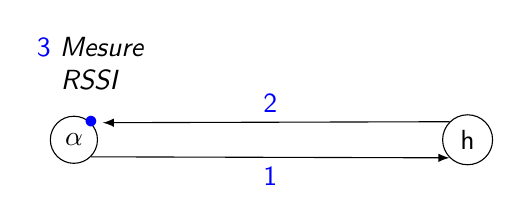
\begin{tikzpicture}
    \node[draw, circle] (A) at (0, 0) {$\alpha$} ;
    \node[draw, circle] (H) at (5, 0) {h} ;

    \draw[->, >=latex] (A.south east) to node[midway, below] {\textcolor{blue}{1}} (H.south west);
    \draw[->, >=latex, shorten >= 1.5mm] (H.north west) to node[midway, above] {\textcolor{blue}{2}} (A.north east);
    \draw (A.north east) node[blue]{$\bullet$} node[above=3mm, align=center] {\textcolor{blue}{3} \textit{Mesure}\\\textit{RSSI}};
  \end{tikzpicture}
\end{center}

Dans le répertoire est aussi présent un fichier Python appelé
\path{read_and_write_to_file.py} qui écoute la ligne série du Wismote avec
\verb+alpha.wismote+ et écrit les valeurs de RSSI mesurées dans un fichier. On
effectue ces mesures sur les 6 cas possibles en plaçant dans chacun des cas les
nœuds de références $A, B, C$ à leur position effective pour la
trilatération\footnote{Pour ainsi essayer d'avoir le coefficient $\alpha$ le
plus juste possible.}. On les stocke dans 6 fichiers différents que nous
utiliserons plus tard.

En ce qui concerne le coefficient $\beta$, on peut aussi s'attendre à ce que ce
dernier soit différent en fonction des cas. Un capteur peut être placé d'une
mauvaise manière de telle sorte que la qualité de la propagation diminue par
rapport à un autre capteur. On reviendra plus tard sur la détermination de ces
coefficients.

\paragraph{Phase d'initialisation : distances entre les nœuds fixes}

En regardant les formules du \autoref{th:base-plan}, on remarque que l'on a
besoin des distances entre les trois points de références $A, B, C$ pour
calculer notre repère orthonormée. Avant la trilatération effective, il nous
faut donc une phase d'initialisation qui mesure les RSSI entre ces points. Nous
proposons la méthode suivante :

\begin{center}
  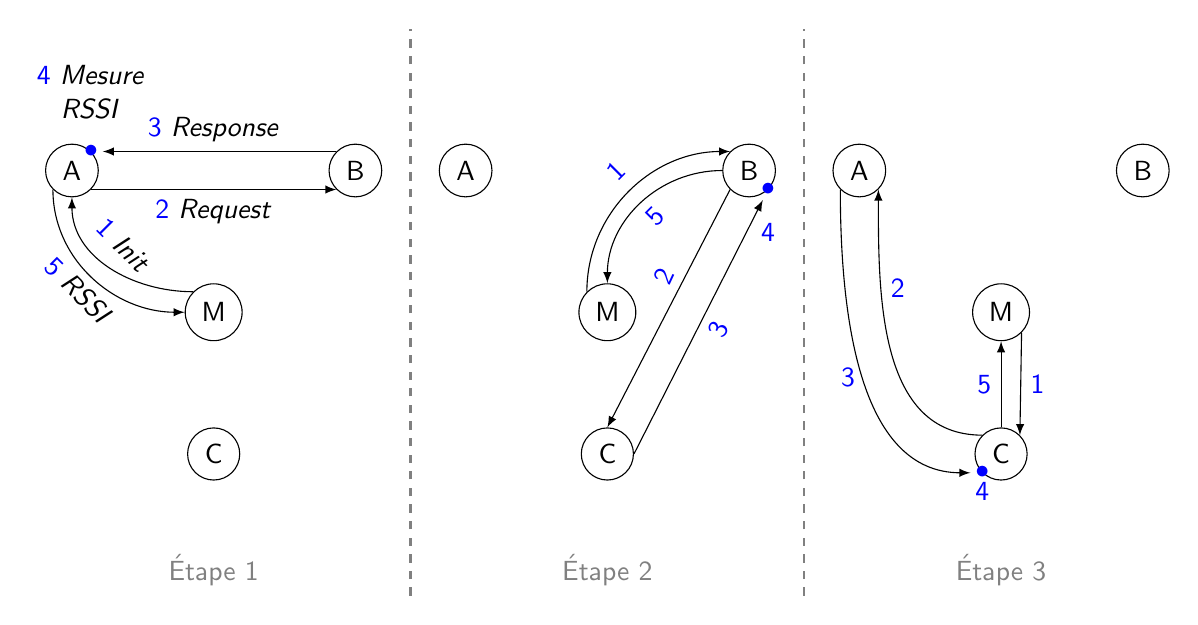
\begin{tikzpicture}
    \def\h{1.8};
    \def\L{5};

    % Étape 1
    \node[draw, circle] (M) at (0, 0) {M} ;
    \node[draw, circle] (A) at (-\h, \h) {A} ;
    \node[draw, circle] (B) at (\h, \h) {B} ;
    \node[draw, circle] (C) at (0, -\h) {C} ;

    \draw[->, >=latex] (M.north west) to[out=180, in=-90] node[midway, above=1mm, rotate=-45] {\textcolor{blue}{1} \textit{Init}} (A.south);
    \draw[->, >=latex] (A.south east) to node[midway, below] {\textcolor{blue}{2} \textit{Request}} (B.south west);
    \draw[->, >=latex, shorten >= 1.5mm] (B.north west) to node[midway, above] {\textcolor{blue}{3} \textit{Response}} (A.north east);
    \draw (A.north east) node[blue]{$\bullet$} node[above=3mm, align=center] {\textcolor{blue}{4} \textit{Mesure}\\\textit{RSSI}};
    \draw[->, >=latex] (A.south west) to[out=-90, in=180] node[midway, below, rotate=-45] {\textcolor{blue}{5} \textit{RSSI}} (M.west);
    
    % Étape 2
    \node[draw, circle] (M2) at (\L, 0) {M} ;
    \node[draw, circle] (A2) at (\L-\h, \h) {A} ;
    \node[draw, circle] (B2) at (\L+\h, \h) {B} ;
    \node[draw, circle] (C2) at (\L, -\h) {C} ;

    \draw[->, >=latex] (M2.north west) to[out=90, in=180] node[midway, above=1mm, rotate=45] {\textcolor{blue}{1}} (B2.north west);
    \draw[->, >=latex] (B2.south west) to node[pos=0.4, above, rotate=65] {\textcolor{blue}{2}} (C2.north);
    \draw[->, >=latex, shorten >= 1.5mm] (C2.east) to node[midway, below, rotate=65] {\textcolor{blue}{3}} (B2.south east);
    \draw (B2.south east) node[blue]{$\bullet$} node[below=3mm] {\textcolor{blue}{4}};
    \draw[->, >=latex] (B2.west) to[out=180, in=90] node[midway, below, rotate=45] {\textcolor{blue}{5}} (M2.north);

    % Étape 3
    \node[draw, circle] (M3) at (2*\L, 0) {M} ;
    \node[draw, circle] (A3) at (2*\L-\h, \h) {A} ;
    \node[draw, circle] (B3) at (2*\L+\h, \h) {B} ;
    \node[draw, circle] (C3) at (2*\L, -\h) {C} ;

    \draw[->, >=latex] (M3.south east) to node[midway, right] {\textcolor{blue}{1}} (C3.north east);
    \draw[->, >=latex] (C3.north west) to[out=180, in=-90] node[pos=0.7, right] {\textcolor{blue}{2}} (A3.south east);
    \draw[->, >=latex, shorten >= 1.5mm] (A3.south west) to[out=-90, in=180] node[midway, left] {\textcolor{blue}{3}} (C3.south west);
    \draw (C3.south west) node[blue]{$\bullet$} node[below] {\textcolor{blue}{4}};
    \draw[->, >=latex] (C3.north) to node[midway, left] {\textcolor{blue}{5}} (M3.south);

    % Sép
    \draw[dashed, gray, thick] (\L/2, -2*\h) -- (\L/2, 2*\h) ;
    \draw[dashed, gray, thick] (3*\L/2, -2*\h) -- (3*\L/2, 2*\h) ;
    \draw[gray] (0, -2*\h) node[above] {Étape \no1} ;
    \draw[gray] (\L, -2*\h) node[above] {Étape \no2} ;
    \draw[gray] (2*\L, -2*\h) node[above] {Étape \no3} ;
  \end{tikzpicture}
\end{center}

Pour chaque point de référence :
\begin{enumerate}
  \item le point $M$ envoie un message \textit{unicast} au point de référence
    avec le \textit{payload} \og{}Initialisation\fg{} ; 
  \item le point de référence envoie un message \textit{unicast} au point de
    référence qui suit avec le \textit{payload} \og{}Request\fg{} ; 
  \item le second point de référence répond avec un message \textit{unicast}
    avec le \textit{payload} \og{}Response\fg{} ; 
  \item à la réception de ce message, le point de référence mesure le RSSI ; 
  \item enfin, il renvoie la valeur au point $M$. 
\end{enumerate}

\begin{remark}
  On retrouve trois des 6 cas de mesure de RSSI mentionnés au paragraphe
  précédent.
\end{remark}

On répète ces trois mesures autant de fois que l'on peut. Dans le code source
\verb+git+ de notre projet se trouve le répertoire
\path{code/trilateration/init} implémentant cette initialisation, avec en
particulier trois fichiers :
\begin{itemize}
  \item \verb+localizor.c+ : code C à programmer sur les nœuds correspondant
    aux points de référence $A, B, C$ ;
  \item \verb+node_to_localize.c+ : code C à programmer sur le nœud
    représentant le point $M$. Ce code envoie le message
    \og{}Initialisation\fg{} périodiquement (tous les intervalles de temps
    donnés par \verb+INITIALISATION_INTERVAL+) et à tour de rôle aux points de
    référence ($A$, puis $B$, puis $C$, puis $A$, \textit{etc.}), et affiche
    sur \verb+stdout+ les valeurs de RSSI qu'on lui a envoyées ;
  \item \verb+deploy.sh+ : un script qui demande les identifiants constructeurs
    des nœuds et qui déploie les codes dans les Wismote correspondants
    (utilisation : \verb+./deploy.sh flash+).
\end{itemize}

Dans le même répertoire, le fichier Python appelé
\path{read_and_write_to_file.py} écoute la ligne série du Wismote $M$. Il écrit
les valeurs de RSSI mesurées dans un fichier, avec une ligne correspondant à 3
mesures de RSSI, une pour chacun des points $A, B, C$.

\paragraph{Phase principale : distances entre le nœud à localiser et les nœuds fixes}

Avec ce qui précède, il ne reste plus qu'à mesurer les distances entre le point
que l'on cherche à localiser et les 3 points de références pour ainsi en
déduire la position de $M$. Le principe est très simple : on mesure les valeurs
de RSSI issues des signaux des trois points $A, B, C$, et ce de manière
périodique :

\begin{center}
  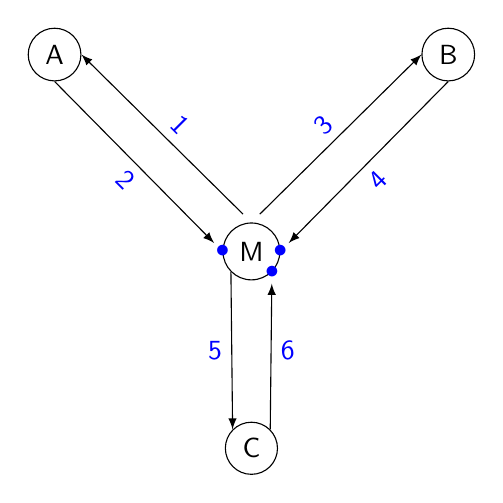
\begin{tikzpicture}
    \def\h{2.5};

    \node[draw, circle] (M) at (0, 0) {M} ;
    \node[draw, circle] (A) at (-\h, \h) {A} ;
    \node[draw, circle] (B) at (\h, \h) {B} ;
    \node[draw, circle] (C) at (0, -\h) {C} ;

    \draw[->, >=latex, shorten <= 1.5mm] (M.north) to node[midway, above, rotate=-45] {\textcolor{blue}{1}} (A.east);
    \draw[->, >=latex, shorten >= 1.5mm] (A.south) to node[midway, below, rotate=-45] {\textcolor{blue}{2}} (M.west) node[blue]{$\bullet$};
    \draw[->, >=latex, shorten <= 1.5mm] (M.north) to node[midway, above, rotate=45] {\textcolor{blue}{3}} (B.west);
    \draw[->, >=latex, shorten >= 1.5mm] (B.south) to node[midway, below, rotate=45] {\textcolor{blue}{4}} (M.east) node[blue]{$\bullet$};
    \draw[->, >=latex] (M.south west) to node[midway, left] {\textcolor{blue}{5}} (C.north west);
    \draw[->, >=latex, shorten >= 1.5mm] (C.north east) to node[midway, right] {\textcolor{blue}{6}} (M.south east) node[blue]{$\bullet$};
  \end{tikzpicture}
\end{center}

Le nœud $M$ envoie un message \textit{unicast} sans \textit{payload} aux 3
capteurs à tour de rôle qui lui répondent immédiatement. À la réception du
signal, le point $M$ mesure la valeur du RSSI.

\begin{remark}
  On retrouve les 3 derniers cas manquants pour la mesure de $\alpha$.
\end{remark}

La phase principale de la trilatération est implémenté dans le code \verb+git+
dans le répertoire \path{code/trilateration/main}. Il contient :
\begin{itemize}
  \item \verb+localizor.c+ : code C à programmer sur les nœuds correspondant
    aux points de référence $A, B, C$ (code plus simple et distinct de la
    partie précédente);
  \item \verb+node_to_localize.c+ : code C à programmer sur le nœud
    représentant le point $M$. Ce code effectue les 3 mesures de RSSI tous les
    intervalles de temps donnés par \verb+RETREIVE_ALL_RSSI_INTERVAL+.
    L'intervalle de temps entre les 3 mesures est donnée par
    \verb+ASK_RSSI_INTERVAL+. Le code affiche sur \verb+stdout+ les valeurs de
    RSSI qu'on lui a envoyées ;
  \item \verb+deploy.sh+ : un script qui demande les identifiants constructeurs
    des nœuds et qui déploie les codes dans les Wismote correspondants
    (utilisation : \verb+./deploy.sh flash+).
\end{itemize}

Comme dans les parties précédentes, on sauvegarde les valeurs de RSSI trouvées
et affichées par $M$ dans un fichier grâce à un script Python
\path{read_and_write_to_file.py} qui met sur chacune des lignes les RSSI des
trois points mesurés.

\subsubsection{Résultats et performances}

Maintenant qu'on a toutes les données pour faire de la trilatération, on peut
écrire un script Python qui affiche sur un graphe les coordonnées des points du
nœud à localiser. Ce programme se base sur les trois étapes ci-dessus :
\begin{itemize}
  \item il lit les 6 fichiers contenant les RSSI à $1$ mètre pour en déduire
    les valeurs de $\alpha$ ;
  \item il lit le fichier contenant les RSSI entre les 3 points de référence
    $A, B, C$ pour en déduire les distances entre eux puis les coordonnées du
    repère du \autoref{th:base-plan} ainsi que la matrice $P$ du
    \autoref{th:trilat-plan} ;
  \item il lit le fichier principal contenant les RSSI entre le point $M$ à
    localiser et les points de référence, en déduit les distances, puis calcule
    avec le vecteur $U$ la position du point $M$ dans le repère. Enfin, il
    affiche sur un graphe les différentes positions calculées.
\end{itemize}

Le script Python se trouve dans notre code source dans le répertoire
\path{code/trilateration/graphe}. On trouvera aussi dans ce répertoire les
différents fichiers contenant les RSSI pour une série de mesure réalisée dans
l'amphithéâtre Thévenin (\textit{cf.} \autoref{fig:amphi}).

\begin{figure}[h!]
    \centering
    \includegraphics[width=0.9\textwidth]{amphi-rouge.jpeg}
    \caption{Environnement où les mesures ont été faites. Les points rouges
    sont la position des nœuds de référence $A, B, C$ dans l'ordre de gauche à
    droite.}
    \label{fig:amphi}
\end{figure}

L'utilisation du script Python, appelé \path{graphe.py}, est décrite par la
commande suivante :
\begin{minted}[frame=single, breaklines]{text}
python graphe.py --help
usage: graphe.py [-h] [-n] [-m] [-v] [-t] filename

positional arguments:
  filename    nom du fichier contenant les RSSI du point à localiser

options:
  -h, --help  show this help message and exit
  -n          rend l'ordonnée de C négative
  -m          utilise la moyenne au lieu de la médiane
  -v          verbose : affiche des données supplémentaires sur le stdout
  -t          affiche la trajectoire au lieu d'un nuage de points
\end{minted}

En particulier, on trouve l'option \verb+-n+ précisant si l'ordonnée de $C$ dans
le \autoref{th:base-plan} est négative ou non selon si notre placement dans
l'amphithéâtre des nœuds de référence correspond à un triangle orienté
positivement ou non. On précise avec le paramètre \verb+filename+ le nom du
fichier qui contient les RSSI entre le point $M$ et les nœuds de référence. Le
nom des autres fichiers est précisé directement dans le script Python, et ils
sont à changer si besoin en fonction des cas. L'option \verb+-m+ précise qu'il
faut utiliser la moyenne au lieu de la médiane pour le calcul des coefficients
$\alpha$ et des distances de référence $AB, BC$ et $AC$. Les RSSI obtenus
pouvant quelques fois donner des valeurs aberrantes très loin de la moyenne, la
médiane nous semble plus pertinente à utiliser. L'option \verb+-t+ est juste une
option d'affichage, et \verb+-v+ affiche des moyennes et des écart-types sur les
données.

On a effectué 3 séries de mesures : deux où l'on marche en ligne droite durant
les mesures (\textit{cf.} \autoref{fig:amphi-tr-droit}), et une où l'on est fixe
(\textit{cf.} \autoref{fig:amphi-tr-fixe}).

\begin{figure}[p]
    \centering
    \includegraphics[width=0.9\textwidth]{amphi-orange.jpeg}
    \caption{Trajectoire de la ligne droite pour les deux séries de mesure
    \texttt{ligne\_droite.csv} et \texttt{ligne\_droite2.csv}.}
    \label{fig:amphi-tr-droit}
\end{figure}

\begin{figure}[p]
    \centering
    \includegraphics[width=0.9\textwidth]{amphi-orange2.jpeg}
    \caption{Position fixe pour la série de mesure \texttt{point\_fixe.csv}.}
    \label{fig:amphi-tr-fixe}
\end{figure}

Il nous reste un détail à traiter avant de pouvoir utiliser le script Python :
déterminer la valeur de $\beta$. L'article \cite{RSSI} nous dit que cette valeur
se situe entre $\np{1.6}$ et $\np{1.8}$. Cependant, faire tourner notre script
avec $\beta=\np{1.7}$ ne marche pas et nous donne un calcul d'une racine carrée
négative lors du calcul de l'ordonnée de $C$. Nous pensons qu'il est intéressant
d'attribuer de la même manière que $\alpha$ des valeurs différentes de $\beta$
selon les cas. En particulier, du fait de l'environnement, nous avons eu du mal
à placer le capteur $C$ d'une manière optimale pour la propagation (il était
gêné par des fils) par rapport aux deux autres capteurs, et mettre une valeur de
$\beta$ supérieure permet de prendre en compte ce problème. À la fin, nous avons
choisi les valeurs suivantes pour $\beta$ qui nous paraissent bien et donnent
des distances cohérentes pour $AB, BC$ et $AC$ :
\begin{minted}[frame=single, breaklines]{python}
betas = {
        "M<-A": 1.5,
        "M<-B": 1.5,
        "M<-C": 2.7,
        "A<-B": 1.5,
        "B<-C": 1.5,
        "C<-A": 2.7,
        }
\end{minted}

Appliquons notre script à la première série de mesures, avec la commande :
\begin{minted}[frame=single, breaklines]{text}
python graphe.py -n -v ligne_droite.csv
\end{minted}

On obtient le graphe suivant :
\begin{center}
  \includegraphics[width=0.9\textwidth]{trilat1.png}
\end{center}

On est loin d'avoir une ligne droite. L'option verbose \verb+-v+ nous donne des
éléments d'explication de pourquoi la trilatération ne semble pas marcher :
\begin{minted}[frame=single, breaklines]{text}
Moyenne RSSI AM : -41.877778 dBm
Médiane RSSI AM : -41.000000 dBm
Écart-type RSSI AM : 4.364895 dBm
Écart de distance AM Moyenne / Moyenne - Écart-type : 8.032926
Écart de distance AM Moyenne / Moyenne + Écart-type : 4.110368

Moyenne RSSI BM : -40.122222 dBm
Médiane RSSI BM : -40.000000 dBm
Écart-type RSSI BM : 6.445672 dBm
Écart de distance BM Moyenne / Moyenne - Écart-type : 10.863504
Écart de distance BM Moyenne / Moyenne + Écart-type : 4.038857

Moyenne RSSI CM : -44.966667 dBm
Médiane RSSI CM : -43.500000 dBm
Écart-type RSSI CM : 9.561686 dBm
Écart de distance CM Moyenne / Moyenne - Écart-type : 6.917148
Écart de distance CM Moyenne / Moyenne + Écart-type : 3.060487
\end{minted}

Ces valeurs montrent qu'un écart de $\sigma$ autour de la moyenne des RSSI peut
donner jusqu'à un écart de $\np{10.86}$ mètres, soit la largeur de
l'environnement où a été réalisé les mesures. Nos valeurs de RSSI mesurées
semblent alors être trop éparpillées les unes des autres. La seconde série de
mesure \path{ligne_droite2.csv} donne malheureusement aussi des résultats
similaires :
\begin{center}
  \includegraphics[width=0.9\textwidth]{trilat2.png}
\end{center}

Mais pour la série de mesure où le point est fixe, on obtient des résultats
plus satisfaisants :
\begin{center}
  \includegraphics[width=0.9\textwidth]{trilat3.png}
\end{center}
On arrive à obtenir un point fixe, mais le point obtenu ne correspond pas à la
réelle position de la \autoref{fig:amphi-tr-fixe}.

Ces deux cas expliquent pourquoi la trilatération n'est pas efficace dans notre
cas :
\begin{itemize}
  \item les mesures en ligne droite montrent que les valeurs de RSSI mesurées
    sont trop imprécises, ce qui affecte directement le modèle de propagation
    qui dépend exponentiellement en les mesures de RSSI. Ces imprécisions
    peuvent venir directement des capteurs des Wismote ou bien de
    l'environnement de travail : l'amphithéâtre Thévenin est soumis aux
    interférences des routeurs Wi-Fi de la salle. En particulier, les ondes
    émises par les Wismote ont des fréquences comprises entre \np{2.394} et
    \np[GHz]{2.507} \footnote{D'après
    \url{https://www.ti.com/lit/ds/symlink/cc2520.pdf}, section 16.} tandis que
    l'une des bandes du Wi-Fi est la bande \np[GHz]{2,4} \footnote{\textit{Cf.}
    \url{https://fr.wikipedia.org/wiki/Liste_des_canaux_Wi-Fi}.}; 
  \item dans les cas où l'on arrive à des mesures précises qui ne s'éparpillent
    pas comme dans le cas du point fixe, la position du point est incohérente,
    signifiant des valeurs de $\alpha$ et/ou $\beta$ mal calibrées. Du moins,
    nos valeurs permettent d'obtenir un repère orthonormé avec une position
    correcte pour les points $A, B$ et $C$.
\end{itemize}

\subsection{Conclusion sur la pertinence de la méthode de la trilatération et pistes d'amélioration}

La trilatération propose un cadre mathématique très rigoureux en ce qu'il donne
des formules explicites pour la résolution du problème de la localisation.
Cependant, en pratique, cette méthode a du mal à faire ses preuves comme vu
avec les résultats ci-dessus. Elle est lourde en ce qu'elle nécessite de la
calibration avec le calcul de $\alpha$ et une phase d'initialisation pour
calculer la distance entre les capteurs de référence. Elle est fortement
dépendante du modèle de propagation proposé, et si ce dernier n'est pas adapté,
alors les positions ne sont pas précises ni correctes. La méthode de
\textit{fingerprinting} présentée dans la section suivante donne des résultats
plus satisfaisants, et n'a pas les contraintes de calcul de distances ni
d'utilisation d'un modèle de propagation dépendant de constantes à déterminer.

\section{Empreinte radio (\textit{fingerprinting})}

\subsection{Principe}

\subsubsection{Empreinte radio de la salle}

Pour réaliser de la géolocalisation intérieure, la méthode de l'empreinte radio
ou \textit{fingerprinting} consiste à recueillir pour un ensemble de points
donnés les valeurs de RSSI en ces points. Ensuite, la localisation du point $M$
est déduite en comparant les RSSI mesurés au point $M$ aux différents RSSI des
points de référence. Le point ayant les RSSI les plus proches au point $M$ donne
sa localisation \cite{FP}.

\subsubsection{Quelques notions d'apprentissage supervisé}

Il nous semble important de mentionner (rapidement) la notion d'apprentissage
supervisé en ce qu'elle va être utile pour le \textit{fingerprinting}.

Soit $S_n = \left\lbrace (x_i, y_i)\,|\,i\in[\![1, n]\!]\right\rbrace$
l'ensemble d'entraînement, où les $(x_i)$ sont des échantillons et les $(y_i)$
les étiquettes associées aux échantillons. Par exemple, $x_i$ peut représenter
un mail, et $y_i$ identifie si c'est du spam ou non. Le but de l'apprentissage
supervisé est de trouver une fonction optimale de prédiction $f$ qui à un
échantillon en dehors de l'ensemble d'entraînement associe une prédiction de sa
classe $y$. En reprenant le même exemple, la fonction de prédiction apprise à
partir des mails reçus précédemment permet de détecter si un nouveau mail est du
spam ou non.

Dans notre cas, on peut faire un lien directe avec l'apprentissage supervisé en
considérant :
\begin{itemize}
  \item $S_n$ notre base de données où l'on a recueilli $n$ fois les valeurs de
    RSSI pour un point donné ;
  \item $x_i = \left(x_i^1, \dotsc, x_i^p\right)$ un échantillon de $p$ valeurs
    de RSSI par rapport à $p$ nœuds $A_1, \dotsc, A_p$ ;
  \item $y_i$ l'étiquette donnant le point où a été réalisé les $p$ mesures de
    RSSI de l'échantillon $i$.
\end{itemize}

Notre but est de trouver grâce à l'empreinte des RSSI des points de référence
une fonction $f$ qui prédit le mieux la position du point $M$ à partir de ses
$p$ mesures de RSSI. La théorie de l'apprentissage supervisé va nous permettre
de nous donner les algorithmes de détermination des fonctions de prédiction
sans que l'on ait a les implémentés. Il existe en ce sens une librairie Python
appelée \verb+scikit-learn+ donnant accès aux algorithmes d'apprentissage
supervisé. On reviendra plus tard sur les algorithmes utilisés.

\subsection{Implémentation}

\subsubsection{Implémentation avec les nœuds Wismote sous Contiki OS}

Le code à implémenter est beaucoup plus simple que pour la trilatération car
cette fois-ci, il n'y a pas plusieurs étapes d'initialisation où il faut
changer le code des Wismote à chaque fois. Ici, pour le code C, il n'y a qu'un
seul répertoire presque similaire au répertoire de la phase principale pour la
trilatération. Ce répertoire s'intitule \path{code/fingerprinting/wismote} et
contient :
\begin{itemize}
  \item \verb+localizor.c+ : code C à programmer sur les nœuds $A_1,\dotsc,A_p$ ;
  \item \verb+node_to_localize.c+ : code C à programmer sur le nœud représentant
    le point $M$ collectant les RSSI / à localiser. Ce code effectue des mesures
    de RSSI par rapport aux $p$ nœuds tous les intervalles de temps donnés par
    \verb+RETREIVE_ALL_RSSI_INTERVAL+. L'intervalle de temps entre les $p$
    mesures est donnée par \verb+ASK_RSSI_INTERVAL+. Le code affiche sur
    \verb+stdout+ les valeurs de RSSI mesurées ;
  \item \verb+deploy.sh+ : un script qui demande les identifiants constructeurs
    des nœuds et qui déploie les codes dans les Wismote correspondants
    (utilisation : \verb+./deploy.sh flash+).
\end{itemize}

\begin{remark}
  Notre code est spécifique à $p=3$. Il aurait été plus intéressant de demander
  dans le script \verb+deploy.sh+ la valeur de $p$ souhaitée et adapter le code
  de \verb+node_to_localize.c+, mais faute de temps, nous nous sommes
  restreints à n'utiliser que 3 nœuds. Ceci étant dit, implémenter $p$ capteurs
  permet indirectement d'implémenter $q<p$ capteurs si l'on ignore certains
  nœuds. On pourrait donc regarder les cas $p=1$ et $p=2$, mais cela nous fait
  perdre de l'information et donc de la précision.
\end{remark}

La communication des Wismote est ainsi identique à la phase principale de la
trilatération, à la différence près que le nombre de nœuds n'est pas
nécessairement 3. Dans le même répertoire, on fournit deux scripts Python :
\begin{itemize}
  \item un script pour l'empreinte radio de la salle. Ce script s'appelle
    \path{training_file_creator.py} et écrit sur un fichier les valeurs de RSSI
    mesurée et lues sur le \verb+stdout+ du lien série du point $M$. Il n'est
    pas à utiliser directement, \textit{cf.} la suite ;
  \item un script pour les mesures pour la localisation du point $M$. Il est
    très similaire au script précédent, et est à utiliser directement. Il
    s'appelle \path{test_file_creator.py}.
\end{itemize}

Nous avons décidé de réaliser une empreinte radio suivant un quadrillage
rectangulaire avec des points espacés d'un mètre\footnote{On a utilisé un câble
d'un mètre pour séparer les points.}. Chaque point de notre quadrillage est
identifié par un couple d'entier $(i, j)$ :
\begin{center}
    \begin{tikzpicture}
      % Axes
      \draw[->] (-1, 0) -- (6, 0) node[anchor=north west]{$i$};
      \draw[->] (0, -1) -- (0, 4) node[anchor=north east]{$j$};
      \draw (0, 0) node[anchor=north east]{$0$};
  
      \def\e{0.1}
      \draw (1, -\e) node[below]{$1$} -- (1, \e);
      \draw (2, -\e) node[below]{$2$} -- (2, \e);
      \draw (3, -\e) node[below=1mm]{$\dotso$};
      \draw (5, -\e) node[below]{$i_{\max}$} -- (5, \e);

      \draw (-\e, 1) node[left]{$1$} -- (\e, 1);
      \draw (-\e, 2) node[left=1mm]{$\vdots$};
      \draw (-\e, 3) node[left]{$j_{\max}$} -- (\e, 3);

      % Points
      \foreach \i in {1,...,5} {
        \foreach \j in {1,...,3} {
          \draw (\i-\e, \j) -- (\i+\e, \j);
          \draw (\i, \j-\e) -- (\i, \j+\e);
        };
      };
    \end{tikzpicture}
\end{center}

Dans les graphes qui suivent, l'axe $j$ est inversé à cause d'une erreur dans
l'ordre de réalisation de nos mesures pour l'empreinte radio. Cette erreur, mis
à part l'axe inversé, est sans importance pour la suite.
\begin{center}
    \begin{tikzpicture}
      % Axes
      \draw[->] (-1, 0) -- (6, 0) node[anchor=north west]{$i$};
      \draw[->] (0, 4) -- (0, -1) node[anchor=north east]{$j$};
  
      \def\e{0.1}
      \draw (1, -\e) node[below]{$1$} -- (1, \e);
      \draw (2, -\e) node[below]{$2$} -- (2, \e);
      \draw (3, -\e) node[below=1mm]{$\dotso$};
      \draw (5, -\e) node[below]{$i_{\max}$} -- (5, \e);

      \draw (-\e, 3) node[left]{$1$} -- (\e, 3);
      \draw (-\e, 2) node[left=1mm]{$\vdots$};
      \draw (-\e, 1) node[left]{$j_{\max}$} -- (\e, 1);

      % Points
      \foreach \i in {1,...,5} {
        \foreach \j in {1,...,3} {
          \draw (\i-\e, \j) -- (\i+\e, \j);
          \draw (\i, \j-\e) -- (\i, \j+\e);
        };
      };
    \end{tikzpicture}
\end{center}

Le script \path{measure_training_set.sh} automatise l'écriture d'un fichier
contenant les RSSI de chaque point du quadrillage. Il demande au début la valeur
de $i_{\max}$ et de $j_{\max}$ puis pour chaque couple $(i, j)$, exécute le
script \path{training_file_creator.py}. Ce dernier indique le couple $(i, j)$
puis écrit les mesures de RSSI lues jusqu'à ce qu'on appuie sur \verb+C-C+.
Après cela, le script passe au couple suivant. À la fin, on obtient un fichier
comme celui-ci :
\begin{minted}[frame=single, breaklines]{text}
c 1 1
129.0: -27,145.0: -56,36.0: -42,
129.0: -28,145.0: -48,36.0: -42,
...
c 1 2
129.0: -38,145.0: -46,36.0: -43,
129.0: -44,145.0: -42,36.0: -54,
...
c 1 3
129.0: -31,145.0: -45,36.0: -39,
129.0: -32,145.0: -40,36.0: -46,
...
\end{minted}

Nous avons réalisé l'empreinte radio dans la même salle que pour la
trilatération. On a identifié au sol le quadrillage à l'aide de petits papiers
et du câble de $1$ mètre pour l'espacement entre les points. La
\autoref{fig:amphi-bleu} donne un tel quadrillage. Comme dit plus haut, on a
pris $p=3$, et les capteurs ont été positionnés aux mêmes endroits que pour la
trilatération (de telle sorte à pouvoir comparer les deux méthodes).

\begin{figure}[h]
    \centering
    \includegraphics[width=0.9\textwidth]{amphi-bleu.jpeg}
    \caption{Quadrillage représenté par les points bleus. L'axe des $i$ va de
    bas en haut, et l'axe des $j$ de gauche à droite. Ici $(i_{\max}, j_{\max})
    = (12, 3)$.}
    \label{fig:amphi-bleu}
\end{figure}

Après avoir réalisé l'empreinte radio, on effectue les mesures de RSSI pour le
point à localiser à l'aide du script Python \path{test_file_creator.py}. On a
décidé de réaliser les mesures sur les deux mêmes cas que pour la trilatération
:
\begin{itemize}
  \item une trajectoire de ligne droite identique à la
    \autoref{fig:amphi-tr-droit} et donnée par les fichiers de mesure
    \path{clean_ligne_droite.csv} et \path{clean_ligne_droite2.csv}. Le premier
    correspond à une trajectoire avec les $i$ croissants, et le second avec les
    $i$ décroissants. Dans les deux cas, on s'est efforcé d'être sur l'axe
    $j=2$ ;
    \item aucune trajectoire avec un point fixe au cours du temps.
      Contrairement à la trilatération, on a fait plus de mesures pour ce cas
      avec 4 positions distinctes données par les figures
      \ref{fig:amphi-fp-o1}, \ref{fig:amphi-fp-o2}, \ref{fig:amphi-fp-o3} et
      \ref{fig:amphi-fp-o4}.
\end{itemize}

\begin{figure}[p]
    \centering
    \includegraphics[width=0.9\textwidth]{amphi-bleu-orange1.jpeg}
    \caption{Position fixe \no1 donnée par le fichier \texttt{clean\_coin.csv}.}
    \label{fig:amphi-fp-o1}
\end{figure}

\begin{figure}[p]
    \centering
    \includegraphics[width=0.9\textwidth]{amphi-bleu-orange2.jpeg}
    \caption{Position fixe \no2 donnée par le fichier \texttt{clean\_coin2.csv}.}
    \label{fig:amphi-fp-o2}
\end{figure}

\begin{figure}[p]
    \centering
    \includegraphics[width=0.9\textwidth]{amphi-bleu-orange3.jpeg}
    \caption{Position fixe \no3 donnée par le fichier \texttt{clean\_coin3.csv}.}
    \label{fig:amphi-fp-o3}
\end{figure}

\begin{figure}[p]
    \centering
    \includegraphics[width=0.9\textwidth]{amphi-bleu-orange4.jpeg}
    \caption{Position fixe \no4 donnée par le fichier \texttt{clean\_coin4.csv}.}
    \label{fig:amphi-fp-o4}
\end{figure}

Les fichiers de mesure sont dans le répertoire
\path{code/fingerprinting/graphe}. Ils commencent tous par \verb+clean_+ car
les fichiers originaux présentaient parfois des lignes avec des RSSI en trop,
ces RSSI étant ceux d'une ligne précédente mais qui ont mis plus de temps que
prévu à arriver au point $M$. Et pour que le programme traçant le graphe
fonctionne, il faut un nombre constant et consistent de RSSI par lignes.

Le programme \path{graphe.py} dans le même répertoire prend en argument le nom
du fichier contenant les RSSI du point à localiser, et affiche un graphe avec
les positions prédites par l'algorithme d'apprentissage supervisé. Cette
fonction implémente deux algorithmes en particulier qui sont décrits dans les
sections suivantes.

\begin{minted}[frame=single, breaklines]{text}
python graphe.py --help
usage: graphe.py [-h] [-k NB_NEIGHBORS] [-n] [-t] filename

positional arguments:
  filename         nom du fichier contenant les RSSI du point à localiser

options:
  -h, --help       show this help message and exit
  -k NB_NEIGHBORS  donne le nombre de plus proche voisins à utiliser dans l'algorithme de même nom (défaut: 1)
  -n               utilise les réseaux de neurones (si non précisé, utilise la méthode des k plus proches voisins)
  -t               affiche la trajectoire au lieu d'un nuage de points
\end{minted}

\subsubsection{Résolution par le point le plus proche dans l'espace des RSSI mesurés}

Sans même parler d'apprentissage supervisé, le point qui conviendrait le plus
pour localiser $M$ serait intituivement celui qui a les écarts de RSSI avec le
point $M$ les plus petits. Cela reviendrait à regarder le point $P$ qui
minimise la quantité :
\[
  d(M, P) = \sum_{j=1}^p \bigl(\mathrm{RSSI}(A_j, M) - \mathrm{RSSI}(A_j, P)\bigr)^2
\]
où $P$ est un point de référence du quadrillage, et $\mathrm{RSSI}(A_j, M)$ est
la valeur du RSSI reçue par le point $M$ et issue d'un signal émis par $A_j$.
On voit que cette quantité est en fait une distance dans l'espace
$\mathbb{R}^p$. On admet (\textit{cf.} plus bas) que ce critère de choix du
point $P$ est un cas particulier de l'algorithme des $k$ plus proches voisins
(algorithme décrit ci-dessous) avec $k=1$.

Pour utiliser ce critère, le programme Python doit être utilisé avec seulement
en argument le nom du fichier. En particulier, il ne faut pas préciser
\verb+-n+ ou \verb+-k k+ avec $k>1$. On peut si l'on veut utiliser \verb+-t+.
Appliquons maintenant l'algorithme à nos différents cas.

\paragraph{Mesures d'une ligne droite}

L'option \verb+-t+ nous permet de voir la trajectoire. On obtient les deux
graphes suivants :
\begin{center}
  \includegraphics[width=0.9\textwidth]{finger1-l1.png}
  \includegraphics[width=0.9\textwidth]{finger1-l2.png}
\end{center}
La trajectoire n'est pas droite du tout, mais grâce au gradient de couleurs, on
peut voir une certaine progression de gauche à droite pour le premier graphe,
et de droite à gauche pour le second. À noter que dans les deux cas, la
trajectoire s'est faite sur l'axe $j=2$, ce qui est loin d'être respecté
surtout pour le second cas. Mais globalement, cela est beaucoup mieux que la
trilatération.

\paragraph{Mesures de positions fixes}

On obtient les quatre graphes suivants :
\begin{center}
  \includegraphics[width=0.9\textwidth]{finger1-f1.png}
  \includegraphics[width=0.9\textwidth]{finger1-f2.png}
  \includegraphics[width=0.9\textwidth]{finger1-f3.png}
  \includegraphics[width=0.9\textwidth]{finger1-f4.png}
\end{center}
La médiane\footnote{Définie ici comme étant la prédiction des médianes des
RSSI.} donne une position satisfaisante pour le premier et quatrième cas, tandis
que les autres cas sont décevants. Voyons voir avec d'autres algorithmes si
l'on peut avoir de meilleurs résultats.

\subsubsection{Résolution par la méthode des plus proches voisins}

La méthode des $k$ plus proches voisins est définie comme suit :
\begin{enumerate}
  \item on regarde les $k$ plus petites distances $d(M, P)$, ce qui nous donne
    $k$ points $P_1, \dotsc, P_k$ ;
  \item on regarde quelle est l'étiquette $(i, j)$ qui apparaît le plus parmi
    les points $P_1, \dotsc, P_k$ ;
  \item on associe à $M$ l'étiquette la plus fréquente.
\end{enumerate}

On voit bien pourquoi le cas $k=1$ correspond à la section précédente : cela
revient à choisir $P$ avec la plus petite distance. Appliquons cet algorithme.
Dans la suite, on ne présente que les graphes avec le $k$ qui nous a semblé le
meilleur.

\paragraph{Mesures d'une ligne droite}

\begin{center}
  \includegraphics[width=0.9\textwidth]{finger2-l1.png}
  \includegraphics[width=0.9\textwidth]{finger2-l2.png}
\end{center}
Dans les deux cas, nous avons pris $k=5$. Pour la première trajectoire, quelque
soit $k$ choisi, on obtient une position de départ pire que dans le cas $k=1$.
Sinon la trajectoire est similaire que précédemment. Pour la seconde
trajectoire, elle semble légèrement moins chaotique et a une progression
droite-gauche, mais ce n'est toujours pas une ligne droite. Le point d'arrivée
est meilleur que pour $k=1$.

\paragraph{Mesures de positions fixes}

\begin{center}
  \includegraphics[width=0.9\textwidth]{finger2-f1.png}
  \includegraphics[width=0.9\textwidth]{finger2-f2.png}
  \includegraphics[width=0.9\textwidth]{finger2-f3.png}
  \includegraphics[width=0.9\textwidth]{finger2-f4.png}
\end{center}

Les valeurs de $k$ choisies sont dans l'ordre $5, 3, 10$ et $5$. Dans les cas
1, 2 et 4, la médiane est très satisfaisante. Elle l'est moins pour le
troisième cas, mais reste meilleur que pour $k=1$.

L'inconvénient de cette méthode est qu'il faut choisir une valeur de $k$, ce
qui peut être fastidieux. Mis à part cela, on arrive à trouver des valeurs de
$k$ qui donnent de meilleurs résultats que $k=1$.

\subsubsection{Résolution par les réseaux de neurones}

Les réseaux de neurones, et en particulier ici les perceptrons à plusieures
couches, sont l'un des algorithmes d'apprentissage supervisé. Nous ne
détaillons pas ici son fonctionnement, et on pourra se référer à la
\href{https://scikit-learn.org/stable/modules/neural\_networks\_supervised.html\#multi-layer-perceptron}{documentation
du module \texttt{scikit-learn}} sur le sujet pour un aperçu de comment cela
marche.

\paragraph{Mesures d'une ligne droite}

\begin{center}
  \includegraphics[width=0.9\textwidth]{finger3-l1.png}
  \includegraphics[width=0.9\textwidth]{finger3-l2.png}
\end{center}
Les trajectoires sont moins bien qu'avec la méthode des plus proches voisins.
En particulier, on déplore la présence du début et de la fin de la trajectoire
au milieu de l'environnement pour la seconde trajectoire.

\paragraph{Mesures de positions fixes}

\begin{center}
  \includegraphics[width=0.9\textwidth]{finger3-f1.png}
  \includegraphics[width=0.9\textwidth]{finger3-f2.png}
  \includegraphics[width=0.9\textwidth]{finger3-f3.png}
  \includegraphics[width=0.9\textwidth]{finger3-f4.png}
\end{center}
Les médianes proposées sont bien pour le premier et dernier cas. Pour les
autres cas, la méthode des $k$ plus proches voisins est préférable.

\subsection{Conclusion sur la pertinence de la méthode de \textit{fingerprinting} et pistes d'amélioration}

La méthode de \textit{fingerprinting} est beaucoup plus satisfaisante que la
trilatération. Pour des points fixes, on arrive à avoir des positions correctes
avec plus ou moins de succès selon les algorithmes d'apprentissage choisis. La
méthode des $k$ plus proches voisins est la plus intéressante. Elle est aussi
pour les trajectoires en ligne droite, bien que dans ce cas, on déplore une
trajectoire un peu chaotique. Du moins, elle propose une certaine progression
de la trajectoire sur l'axe des $i$, au contraire de la trilatération qui
proposait des points s'éparpillant beaucoup. Par ailleurs, cette méthode est
simple à implémenter au niveau du code, mais demande un peu plus de travail en
matière de collection des données, car reposant sur un ensemble d'apprentissage.

D'autres algorithmes d'apprentissage supervisé existent comme les SVM. Il
aurait été intéressant de voir s'ils donnent de meilleurs résultats. Aussi
pouvait-on jouer sur quelques paramètres pour les réseaux de neurones. Par
manque de temps, nous ne l'avons pas fait. Par ailleurs, nous avons fixé $p$ à
3 et il aurait été aussi intéressant d'augmenter ce nombre pour voir si la
précision augmente, au delà des avantages présentés dans la section suivante.

\section{Compléments}

Voici quelques pistes de réflexion qui sont intéressantes mais dont nous
n'avons pas eu le temps de les étudier en détail.

\subsection{Sur le nombre de capteurs de référence et la consommation énergétique}

Plusieurs fois a-t-il été mentionné ci-dessus des variables constantes en C
fixant des intervalles de temps entre les transmissions, comme
\verb+RETREIVE_ALL_RSSI_INTERVAL+ et \verb+ASK_RSSI_INTERVAL+. Nous avons
choisi ces variables de telle sorte à récolter les RSSI le plus rapidement
possible, et ne laisser que peu de latence. Avec ceci, les capteurs sont
sollicités le plus souvent possible, ce qui n'est pas nécessairement optimal
pour la consommation d'énergie.

Ainsi, on aurait pu utiliser plus que 3 capteurs pour la trilatération et
alterner entre différents groupes de 3 capteurs de référence pour ainsi
diminuer la charge individuelle des nœuds (sans perdre en précision car en
gardant les mêmes intervalles de temps entre les transmissions). Les nœuds non
sollicités passent donc en mode veille pendant un instant donné et diminuent
leur consommation. Il y a deux inconvénients à cela : il faut plus de capteurs,
ce qui entraîne un plus haut coût de déploiement et de maintenance ; et le code
du nœud $M$ devient plus complexe car devant changer les adresses des capteurs
à communiquer avec. Aussi l'augmentation de nœuds augmente la consommation
globale et ne doit pas dépasser l'objectif même de diminution de la
consommation individuelle des capteurs.

Cette idée d'avoir plus de nœuds s'applique aussi au \textit{fingerprinting}.
Cela ne concerne pas l'augmentation de $p$. Au contraire, à un nombre $p$ fixé,
on ajoute quelques capteurs en plus, et on alterne le groupe de $p$ capteurs
avec lesquels on fait la mesure des RSSI.

\subsection{Sur le passage à l'échelle (\textit{scalability})}

Tous nos graphes ont été créés localement : on a récupéré des données que l'on
a stockées dans des fichiers, puis on les a utilisées localement pour calculer
les positions. Notre solution n'implémente pas d'envoi et traitement à distance
de la localisation, aspect qui est important selon les cas d'usage. Ainsi, par
exemple, pour le sauvetage lors des incendies, il semble beaucoup plus
intéressant de connaître la position à l'échelle du bâtiment qu'à l'échelle
d'une salle. En ce sens, comme expliqué ci-dessus, la pile Rime n'est pas la
plus adaptée, ou du moins son utilisation doit rester locale.
\href{https://thingsboard.io/}{Thingsboard} est un outil qui pourrait être
utilisé pour proposer une telle décentralisation et même un contrôle à distance
des capteurs selon les problématiques de la section précédente (contrôle des
intervalles de transmissions, passage en veille, contrôle de la consommation,
\textit{etc.}). Mais il est à noter que la création de graphes de localisation
comme nous avons proposée ci-dessus est à implémenter à la main, Thingsboard ne
proposant pas nativement de telles repères.

Sur un autre sujet, il est possible de s'appuyer sur les infrastructures Wi-Fi
existantes plutôt que de déployer des capteurs dédiés. En utilisant les bornes
Wi-Fi et les antennes des appareils portables, il est possible d'économiser sur
les coûts de déploiement et de gestion des capteurs, tout en permettant
d'ajouter un grand nombre d'utilisateurs dans la limite de la capacité du
réseau Wi-Fi. Cependant, il est important de prendre en compte la capacité du
réseau Wi-Fi et de gérer la congestion pour garantir des performances optimales
de localisation pour tous les utilisateurs.

\subsection{Sur l'apprentissage non supervisé}

L'article \cite{RSSI} mentionne l'utilisation d'algorithmes d'apprentissage non
supervisé pour réduire la dimentionnalité du système (avec l'analyse en
composantes spectrales, \textit{PCA} par exemple). Cela signifie dans le cas de
\textit{fingerprinting} trouver des algorithmes qui réduisent la valeur de $p$
sans perdre de l'information. Notre valeur de $p$ que nous avons utilisée étant
faible, nous n'avions pas intérêt à utiliser de l'apprentissage non supervisé.

\newpage

\appendix

\section{Trilatération dans l'espace}
\label{sec:trilat-space}

\subsection{Formules de trilatération}
\label{subsec:trilat-space}

\begin{theorem}[Trilatération dans l'espace]
  Soient $A, B, C, D, M$ cinq points de l'espace. Soient $d_A, d_B, d_C, d_D$
  les distances euclidiennes respectives entre le point $M$ et les quatre
  points $A, B, C, D$. Si les points $A, B, C, D$ ne sont pas coplanaires,
  alors les coordonnées $(x_M, y_M, z_M)$ du point $M$ sont données par :
  \[
    \begin{pmatrix}x_M\\y_M\\z_M\end{pmatrix} = P^{-1}U 
  \]
  où :
  \[
    P = \begin{pmatrix}
      x_B-x_A & y_B-y_A & z_B-z_A \\
      x_C-x_A & y_C-y_A & z_C-z_A \\
      x_D-x_A & y_D-y_A & z_D-z_A
    \end{pmatrix}\qquad\text{et}\qquad U=\frac{1}{2}\begin{pmatrix}
      {d_A}^2 - {d_B}^2 + {OB}^2 - {OA}^2 \\ 
      {d_A}^2 - {d_C}^2 + {OC}^2 - {OA}^2 \\
      {d_A}^2 - {d_D}^2 + {OD}^2 - {OA}^2
    \end{pmatrix}.
  \]
  avec $A=(x_A, y_A, z_A), B=(x_B, y_B, z_B), C=(x_C, y_C, z_C)$ et $O=(0, 0,
  0)$ le centre du repère.
\end{theorem}

\begin{remark}
  $P^{\mathsf{T}}$ est la matrice des vecteurs $\overrightarrow{AB},
  \overrightarrow{AC}, \overrightarrow{AD}$ dans la base canonique de
  $\mathbb{R}^3$.
\end{remark}

\begin{proof}
  Les expressions des distances en fonction des coordonnées des points donnent
  :
  \begin{align*}
    {d_A}^2 &= (x_M - x_A)^2 + (y_M - y_A)^2 + (z_M - z_A)^2 \tag{$L_1$} \\
    {d_B}^2 &= (x_M - x_B)^2 + (y_M - y_B)^2 + (z_M - z_B)^2 \tag{$L_2$} \\
    {d_C}^2 &= (x_M - x_C)^2 + (y_M - y_C)^2 + (z_M - z_C)^2 \tag{$L_3$} \\
    {d_D}^2 &= (x_M - x_D)^2 + (y_M - y_D)^2 + (z_M - z_D)^2. \tag{$L_4$}
  \end{align*}

  En développant :
  \begin{align}
    {d_A}^2 &= {x_M}^2 + {y_M}^2 + {z_M}^2 - 2\left(x_Mx_A + y_My_A + z_Mz_A\right) + \underbrace{{x_A}^2 + {y_A}^2 + {z_A}^2}_{={OA}^2} \tag{$L_1$} \\
    {d_B}^2 &= {x_M}^2 + {y_M}^2 + {z_M}^2 - 2\left(x_Mx_B + y_My_B + z_Mz_B\right) + \underbrace{{x_B}^2 + {y_B}^2 + {z_B}^2}_{={OB}^2} \tag{$L_2$} \\
    {d_C}^2 &= {x_M}^2 + {y_M}^2 + {z_M}^2 - 2\left(x_Mx_C + y_My_C + z_Mz_C\right) + \underbrace{{x_C}^2 + {y_C}^2 + {z_C}^2}_{={OC}^2} \tag{$L_3$} \\
    {d_D}^2 &= {x_M}^2 + {y_M}^2 + {z_M}^2 - 2\left(x_Mx_D + y_My_D + z_Mz_D\right) + \underbrace{{x_D}^2 + {y_D}^2 + {z_D}^2}_{={OD}^2}. \tag{$L_4$}
  \end{align}

  Par combinaison linéaire des lignes, on obtient :
  \begin{align}
    {d_B}^2 - {d_A}^2 &= -2\left((x_B-x_A)x_M + (y_B-y_A)y_M + (z_B-z_A)y_M\right) + {OB}^2 - {OA}^2 \tag{$L_2 - L_1$} \\
    {d_C}^2 - {d_A}^2 &= -2\left((x_C-x_A)x_M + (y_C-y_A)y_M + (z_C-z_A)y_M\right) + {OC}^2 - {OA}^2 \tag{$L_3 - L_1$} \\
    {d_D}^2 - {d_A}^2 &= -2\left((x_D-x_A)x_M + (y_D-y_A)y_M + (z_D-z_A)y_M\right) + {OD}^2 - {OA}^2 \tag{$L_4 - L_1$}
  \end{align}
  c'est-à-dire :
  \begin{align}
    (x_B-x_A)x_M + (y_B-y_A)y_M + (z_B-z_A)z_M &= \frac{1}{2}\left({d_A}^2 - {d_B}^2 + {OB}^2 - {OA}^2\right) \tag{$L_2 - L_1$} \\
    (x_C-x_A)x_M + (y_C-y_A)y_M + (z_C-z_A)z_M &= \frac{1}{2}\left({d_A}^2 - {d_C}^2 + {OC}^2 - {OA}^2\right) \tag{$L_3 - L_1$} \\
    (x_D-x_A)x_M + (y_D-y_A)y_M + (z_D-z_A)z_M &= \frac{1}{2}\left({d_A}^2 - {d_D}^2 + {OD}^2 - {OA}^2\right) \tag{$L_4 - L_1$} 
  \end{align}
  ce qui revient, avec les notations introduites ci-dessus, à :
  \[
    P\begin{pmatrix}x_M\\y_M\\z_M\end{pmatrix} = U.
  \]

  Supposons que les points $A, B, C, D$ ne soient pas coplanaires. Les vecteurs
  $\overrightarrow{AB}, \overrightarrow{AC}, \overrightarrow{AD}$ ne sont donc
  pas coplanaires \textit{i.e.} non linéairement liés, donc $P^{\mathsf{T}}$
  est inversible, et donc $P$ aussi. D'où :
  \[
    \boxed{\begin{pmatrix}x_M\\y_M\\z_M\end{pmatrix} = P^{-1}U}.\qedhere
  \]
\end{proof}

\subsection{Construction d'une base de l'espace à partir de la distance entre quatre points}
\label{subsec:base-space}

\begin{theorem}
  Soient $A, B, C, D$ quatre points de l'espace tels que $AB\not=0$ et tels que
  les points $A, B, C$ ne soient pas alignés (ces points définissent donc un
  plan de l'espace). Soit $\mathrm{sgn}$ la fonction signe. Si $D$ n'est pas
  dans le plan $(ABC)$, alors $\mathcal{B}=\left(\overrightarrow{AB},
  \overrightarrow{AC}, \overrightarrow{AD}\right)$ est une base de
  $\mathbb{R}^3$, et:
  \begin{itemize}
    \item
      si $\mathcal{B}$ est une base directe, alors :
      \[
        D = \begin{pmatrix}
          \dfrac{{AB}^2 + {AD}^2 - {BD}^2}{{AB}^2} \\[4mm]
          \dfrac{{AC}^2 + {AD}^2 - {CD}^2 - 2x_Cx_D}{2y_C} \\[4mm]
          \mathrm{sgn}(y_C)\sqrt{{AD}^2 - {x_D}^2 - {y_D}^2}
        \end{pmatrix} ;
      \]
    \item
      si $\mathcal{B}$ est une base indirecte, alors :
      \[
        D = \begin{pmatrix}
          \dfrac{{AB}^2 + {AD}^2 - {BD}^2}{{AB}^2} \\[4mm]
          \dfrac{{AC}^2 + {AD}^2 - {CD}^2 - 2x_Cx_D}{2y_C} \\[4mm]
          - \mathrm{sgn}(y_C)\sqrt{{AD}^2 - {x_D}^2 - {y_D}^2}
        \end{pmatrix} ;
      \]
  \end{itemize}
  où ces coordonnées dans les deux cas sont celles de $D$ dans la base
  orthonormée de centre $A$ et de vecteurs directeurs
  $\frac{\overrightarrow{AB}}{AB}, \overrightarrow{n}, \overrightarrow{m}$ avec
  $\overrightarrow{n}$ défini par le \autoref{th:base-plan} dans le plan
  $(ABC)$, et $\overrightarrow{m}$ l'un des deux vecteurs normaux unitaires du
  plan $(ABC)$ tel que la base soit directe.

  \begin{center}
    \begin{tikzpicture}[x={(-0.353cm,-0.353cm)}, z={(0cm,1cm)}, y={(1cm,0cm)}, scale=1.5]
      % Nodes
      \node (A) at (0, 0, 0) {};
      \node (B) at (5, 0, 0) {};
      \node (C) at (3.5, 2, 0) {};
      \node (C2) at (3.5, -2, 0) {};
      \node (D) at (2, 3, 2) {};

      % Axes
      \draw[->] (-1, 0, 0) -- (7, 0, 0) node[anchor=north west]{$x$};
      \draw[->] (0, -3, 0) -- (0, 3, 0) node[anchor=south west]{$y$};
      \draw[->] (0, 0, -1) -- (0, 0, 2.5) node[anchor=south east]{$z$};
      \draw (A) node[anchor=south east]{$A$};
      \draw[->, thick] (0, 0, 0) -- (1.5, 0, 0) node[anchor=north]{$\frac{\overrightarrow{AB}}{AB}$};
      \draw[->, thick] (0, 0, 0) -- (0, 1, 0) node[anchor=south]{$\overrightarrow{n}$};
      \draw[->, thick] (0, 0, 0) -- (0, 0, 1) node[anchor=east]{$\overrightarrow{m}$};

      % Le reste
      \draw (B) node {$+$} node[anchor=north west] {$B$};
      \draw (C) node {$+$} node[anchor=north west] {$C$};
      \draw (C2) node {$+$} node[anchor=north east] {$C'$};
      \draw (D) node {$+$} node[anchor=north east] {$D$};

      \draw[dashed] (A) -- (C) -- (B) -- (C2) -- (A);
      \draw[dotted] (A) -- (2, 3, 0) -- (D);
      \draw[gray] (C) -- node[pos=0.25] {$/$} node[pos=0.75] {$/$} (C2);
    \end{tikzpicture}
  \end{center}
\end{theorem}

\begin{proof}
  L'existence du repère est donnée par sa construction ci-dessus et est assurée
  par le fait que $AB\not=0$ (donc $\overrightarrow{n}$ existe par le
  \autoref{th:base-plan}) et que $(ABC)$ soit un plan (donc
  $\overrightarrow{m}$ existe). Le \autoref{th:base-plan} appliqué dans ce plan
  donne alors les coordonnées du point $C$ :
  \[
    C = \begin{pmatrix}
      \dfrac{{AB}^2 + {AC}^2 - {BC}^2}{2AB} \\[4mm]
      \pm\sqrt{{AC}^2 - {x_C}^2} \\[1mm]
      0
    \end{pmatrix}.
  \]

  Le fait que $A, B, C$ ne soient pas alignés assurent que $y_C \not = 0$. En
  effet, dans la base construite, on a $A=(0, 0, 0)$ et $B=(AB, 0, 0)$ donc si
  $y_C = 0$, alors $C$ appartient à la droite $(AB)$.

  Calculons les coordonnées du point $D$. On a :
  \begin{align*}
    {AD}^2 &= {x_D}^2 + {y_D}^2 + {z_D}^2 \\
    {BD}^2 &= \left(x_D-AB\right)^2 + {y_D}^2 + {z_D}^2 \\
    {CD}^2 &= \left(x_D-x_C\right)^2 + \left(y_D-y_C\right)^2 + {z_D}^2
  \end{align*}
  donc :
  \begin{align*}
    {AD}^2 &= {x_D}^2 + {y_D}^2 + {z_D}^2 \\
    {BD}^2 &= {x_D}^2 + {y_D}^2 + {z_D}^2 - 2x_D\,AB + {AB}^2 \\
    {CD}^2 &= {x_D}^2 + {y_D}^2 + {z_D}^2 - 2x_Cx_D - 2y_Cy_D + \underbrace{{y_C}^2 + {z_C}^2}_{={AC}^2}
  \end{align*}

  On soustrait à la première ligne la seconde et aussi la troisième. On obtient
  :
  \begin{align*}
    {AD}^2 - {BD}^2 &= 2x_D\,AB - {AB}^2 \\
    {AD}^2 - {CD}^2 &= 2x_Cx_D + 2y_Cy_D - {AC}^2
  \end{align*}
  d'où :
  \[
      \boxed{x_D = \frac{{AB}^2 + {AD}^2 - {BD}^2}{2AB}} ;
  \]
  \[
      \boxed{y_D = \frac{{AC}^2 + {AD}^2 - {CD}^2 - 2x_Cx_D }{2y_C}}.
  \]

  Ensuite, la toute première équation donne ${z_D}^2 = {AD}^2 - {x_D}^2 -
  {y_D}^2$. L'orientation de la base $\mathcal{B}$ est donnée par le signe du
  déterminant de la matrice des vecteurs $\overrightarrow{AB},
  \overrightarrow{AC}, \overrightarrow{AD}$, c'est-à-dire la matrice :
  \[
    \begin{pmatrix}
      x_B - x_A & x_C - x_A & x_D - x_A \\
      y_B - y_A & y_C - y_A & y_D - y_A \\
      z_B - z_A & y_C - y_A & z_D - z_A
    \end{pmatrix}
    =
    \begin{pmatrix}
      AB & x_C & x_D \\
      0  & y_C & y_D \\
      0  & 0   & z_D
    \end{pmatrix}.
  \]

  Ce déterminant vaut donc $AB\,y_Cz_D$, et son signe est alors
  celui de $y_Cz_D$ (car $AB$ est toujours positif). Ainsi :
  \begin{itemize}
    \item si $\mathcal{B}$ est directe, alors le déterminant est positif donc
      $z_D$ a le même signe que $y_C$. D'où $\boxed{z_D =
      \mathrm{sgn}(y_C)\sqrt{{AD}^2 - {x_D}^2 - {y_D}^2}}$ ;
    \item si $\mathcal{B}$ est indirecte, alors le déterminant est négatif donc
      $z_D$ a le signe opposé de $y_C$. D'où $\boxed{z_D =
      -\mathrm{sgn}(y_C)\sqrt{{AD}^2 - {x_D}^2 - {y_D}^2}}$.\qedhere
  \end{itemize}
\end{proof}

\section{Installation de Contiki OS, compilation et programmation de code sur les plateformes Wismote}
\label{sec:contiki}

\subsection{Installation}
\label{subsec:contiki-install}

Il y a deux méthodes :
\begin{itemize}
  \item installation du répertoire git de Contiki sur une VM Ubuntu LTS ;
  \item installation de InstantContiki : c'est une VM Ubuntu préconfigurée avec
    tous les outils déjà installés, mais la version d'Ubuntu installée est
    vieille.
\end{itemize}

Nous avons choisi la première méthode car préférant avoir une version Ubuntu à
jour. La deuxième méthode demande moins de travail et moins d'installations.

\subsubsection{Installation de Contiki OS et autres outils sur Ubuntu 22.04.4}

On installe Contiki OS avec :

\begin{minted}[frame=single, breaklines]{bash}
sudo apt install git
git clone https://github.com/contiki-os/contiki
\end{minted}

À noter qu'il existe une version plus récente de Contiki, appelé Contiki NG. Il
ne faut pas utiliser cette dernière car elle ne contient pas la plateforme
Wismote.

L'exécutable \verb+mspgcc+ va nous permettre de compiler du code pour les
plateformes Wismote. On compile \verb+mspgcc+ directement depuis la source, car
le package Ubuntu a une version trop vieille qui ne permet pas de compiler.
\verb+stow+ ci-dessous est un utilitaire qui nous sert à rien. Il est juste
présent ci-dessous pour éviter de modifier le script d'installation de
\verb+mspgcc+.

\begin{minted}[frame=single, breaklines, breakafter=/]{bash}
sudo apt update
sudo apt install build-essential stow texinfo

wget https://raw.githubusercontent.com/contiki-ng/contiki-ng/develop/tools/toolchain/msp430/buildmsp.sh
sudo mdkir /usr/local/stow/mspgcc-4.7.4
sudo ./buildmsp.sh
# On ajoute les exécutables dans PATH
echo 'PATH="/usr/local/stow/mspgcc-4.7.4/bin:$PATH"' >> ~/.profile
\end{minted}

On vérifie que l'installation a fonctionné avec \verb+msp430-gcc --version+.

Enfin, on installe un débogueur qui va nous permettre de programmer le code
compilé sur les cartes Wismotes.

\begin{minted}[frame=single, breaklines, breakafter=/]{bash}
sudo apt install libusb-dev libreadline-dev
wget https://github.com/dlbeer/mspdebug/archive/refs/tags/v0.25.zip
cd mspdebug-0.25
make
sudo make install
\end{minted}

Optionnellement, on peut installer \verb+putty+ pour voir le \verb+stdout+ de
nos programmes. Pour l'utiliser, on exécute \verb+sudo putty+, on choisit
\og{}Serial\fg{}, \verb+/dev/ttyUSB0+ et \verb+115200+ pour l'option
\og{}Speed\fg{}. Un autre outil est \verb+screen+ avec
\verb+screen /dev/ttyUSB0 115200+ produisant le même résultat. Dans notre
projet, nous utilisons le \verb+stdout+ pour récupérer certaines données, et
l'outil que nous avons choisi est \verb+pySerial+ : c'est un module Python que
l'on peut installer avec \verb+sudo apt install python3-serial+.

\subsubsection{Installation de InstantContiki3.0}

Si l'on ne veut pas faire ces installations, on peut aussi utiliser
InstantContiki. On télécharge la VM sur
\url{https://sourceforge.net/projects/contiki/files/Instant\%20Contiki/}.
Ensuite, on décompresse le fichier avec \verb+unzip+ (prend deux ou trois
minutes). À l'intérieur du répertoire se trouve des fichiers VMware d'extension
\verb+vmdk+ (et autres). Nous préférons utiliser \verb+virt-manager+ mais ce
dernier ne peut lire les fichiers de VMware directement. Pour régler ce
problème, on exécute :
\begin{minted}[frame=single, breaklines]{bash}
qemu-img convert -O qcow2 Instant_Contiki_Ubuntu_12.04_32-bit.vmdk InstantContiki.qcow2
\end{minted}

Puis on crée une nouvelle VM avec l'option d'installation depuis une image
virtuelle déjà existante, et on choisit \verb+InstantContiki.qcow2+.

\subsection{Compilation et programmation de code sur les plateformes Wismote}
\label{subsec:contiki-usage}

\subsubsection{Compilation}

On se place dans un répertoire donné contenant le code source C, et on exécute :
\begin{minted}[frame=single, breaklines]{bash}
make TARGET=wismote
\end{minted}

Selon les cas, un ou plus fichiers en \verb+*.wismote+ sont créés : ce sont les
binaires à flasher sur les Wismote.

\subsubsection{Programmation}

Supposons que l'on veuille programmer le code compilé \verb+filename.wismote+ sur
une carte donnée. On branche la carte Wismote au Olimex, et on exécute :

\begin{minted}[frame=single, breaklines]{bash}
sudo mpsdebug olimex 'prog filename.wismote'
\end{minted}

\section{Simulation avec l'outil Cooja de Contiki OS}
\label{sec:cooja}

Cooja est un outil directement inclus dans le répertoire git de Contiki OS. Il
permet de simuler sur Ubuntu les nœuds, et ainsi de tester notre code sans
programmer directement les Wismote, ce qui est un peu fastidieux.

Pour l'utiliser, il faut installer quelques programmes :

\begin{minted}[frame=single, breaklines]{bash}
git submodule update --init
sudo apt install ant
\end{minted}

La commande \verb+git submodule+ va probablement échouer car il y a un module
qui n'existe plus sur \verb+github+. Pour régler le problème, on supprime ce module du
répertoire \verb+git+ en suivant les instructions sur
\url{https://gist.github.com/myusuf3/7f645819ded92bda6677}.

Une fois l'installation finie, on lance Cooja avec :
\begin{minted}[frame=single, breaklines]{bash}
cd tools/cooja
ant run
\end{minted}

\printbibliography

\end{document}
